\chapter{Umsetzung des Prototyps}
\label{chap:umsetzung_des_prototyps}

\section{Implementierung der Chrome Erweiterung}

Die Chrome Erweiterung wurde mit der Version Manifest 3 implementiert.
Genutzt wurden ein \textit{Service Worker} ein \textit{Content Script} pro Nachrichtenportal und ein \textit{Popup}.

\paragraph{Service Worker} steuern eine Seite genau dann, wenn ein Service Worker auf dieser Netzwerkanfragen in seinem Namen abfangen kann. 
Der Service Worker kann dann Aufgaben für die Seite innerhalb eines bestimmten Scopes ausführen

Der Lifecycle eines Service Workers ist in folgende Events unterteilt: installing, installed, activating, activated.

Nach Abschluss der Aktivierung steuert der Service Worker die Seite standardmäßig erst 
bei der nächsten Navigation oder Seitenaktualisierung \ref{chrome2025serviceworker}.

\paragraph{Content Scripts} sind Dateien, die im Kontext von Webseiten ausgeführt werden. 
Mit dem standardmäßigen Document Object Model (DOM) können sie Details der Webseiten lesen, die der Browser besucht, 
Änderungen daran vornehmen und Informationen an die übergeordnete Erweiterung weitergeben \ref{chrome2025contentscripts}.

Die Kommunikation mit den Service Worker erfolgt über die Extension-API \textit{runtime}.

\paragraph{Pop-ups} sind Aktionen, bei denen ein Fenster angezeigt wird, über das Nutzer mehrere Erweiterungsfunktionen aufrufen kann. 
Sie werden durch ein Tastenkürzel, durch Klicken auf das Aktionssymbol der Erweiterung oder durch Drücken von chrome.action.openPopup() ausgelöst. 
Pop-ups werden automatisch geschlossen, wenn der Nutzer sich auf einen Bereich des Browsers außerhalb des Pop-ups konzentriert \ref{chrome2025popups}.

\begin{figure}[htbp]
    \begin{center}
        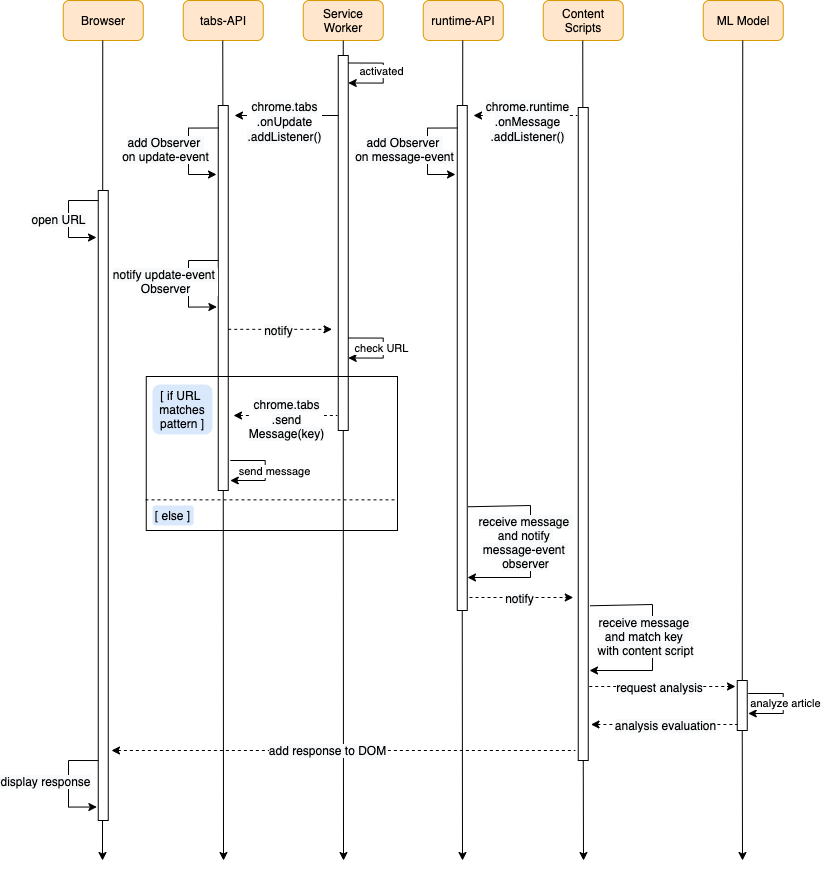
\includegraphics[scale=0.5]{diagrams/hauptkomponente_sequenzdiagramm.png}
        \caption{\label{fig:seq_hauptkomponente} Sequenzdiagramm Hauptkomponente}
    \end{center}
\end{figure}

In Abbildung \ref{fig:seq_hauptkomponente} zu sehen ist das Sequenzdiagramm der Hauptkomponente. Wie in Kapitel \ref{sec:06:hauptkomponente} beschrieben
wird zuerst die URL geprüft. Erfüllt diese die vorgegebenen Bedingungen wird der geöffnete Artikel gelesen und von einer weiteren Anwendung
analysiert. Anschließend wird das Ergebnis der Analyse in einem \textit{div}-Container über dem Artikel eingefügt.

Um die Veränderungen im Browser zu überwachen wurde die \textit{tabs}-API von Chrome genutzt. Anhand dieser kann das Tab-System eines Browsers überwacht
und zum Beispiel auch auf jede Veränderung der URL reagiert werden.
Außerdem ermöglicht die API das Versenden von Nachrichten an alle aktiven Content Scripts. Diese werden dann im jeweiligen Content Script über die
\textit{runtime}-API empfangen und ausgelesen.


